\documentclass[border=4pt]{standalone}
\usepackage{amsmath}
\usepackage{amssymb}
\usepackage{tikz}
\usetikzlibrary{positioning,arrows.meta,fit,calc,shadows}
\begin{document}
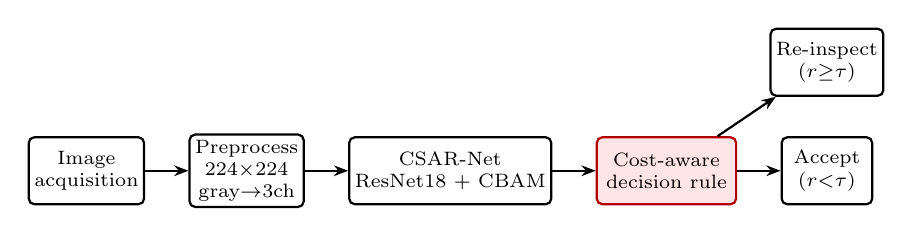
\begin{tikzpicture}[
			box/.style={rectangle,draw,thick,rounded corners=2pt,minimum height=0.85cm,minimum width=1.15cm,font=\scriptsize,align=center,inner sep=2pt},
			key/.style={rectangle,draw=red!70!black,thick,rounded corners=2pt,minimum height=0.85cm,minimum width=1.45cm,font=\scriptsize,align=center,fill=red!10},
			arr/.style={-{Stealth[length=1.8mm]},thick},
		]
			\node[box] (acq) {Image\\acquisition};
			\node[box,right=0.55cm of acq] (pre) {Preprocess\\$224{\times}224$\\gray$\to$3ch};
			\node[box,right=0.55cm of pre] (net) {CSAR-Net\\ResNet18 $+$ CBAM};
			\node[key,right=0.55cm of net] (dec) {Cost-aware\\decision rule};
			\node[box,right=0.55cm of dec] (acc) {Accept\\$(r{<}\tau)$};
			\node[box,above=0.5cm of acc] (re) {Re-inspect\\$(r{\ge}\tau)$};
			\draw[arr] (acq)--(pre);
			\draw[arr] (pre)--(net);
			\draw[arr] (net)--(dec);
			\draw[arr] (dec)--(acc);
			\draw[arr] (dec)--(re);
		\end{tikzpicture}
\end{document}
